\chapter{संरचना के लिए स्पेक्ट्रमिकी}\label{ch:b1:structure-spectroscopy}

एक इत्र-निर्माता प्रयोगशाला को एक रंगहीन द्रव देता है जिससे अनन्नास की गंध आती है,
और पूछता है कि यह क्या है। पचास वर्ष पहले उत्तर पाने में अपघटन अभिक्रियाओं के
कई सप्ताह लग जाते। आज इसमें दस मिनट लगते हैं: एक तत्त्वीय विश्लेषण सूत्र देता है,
एक अवरक्त स्पेक्ट्रम क्रियात्मक समूह का नाम बताता है, और एक प्रोटॉन नाभिकीय
चुंबकीय अनुनाद स्पेक्ट्रम दिखाता है कि परमाणु कैसे जुड़े हैं। यह अध्याय समझाता है
कि हर स्पेक्ट्रम कैसे पढ़ा जाता है --- हर क्षेत्र का प्रकाश अणु के साथ क्या करता है,
और स्पेक्ट्रम की कौन-सी विशेषता संरचना का कौन-सा अंश वहन करती है --- और
अंत में उसी अनन्नास वाले अणु पर पहुँचता है।

\begin{recall}
विद्यालय के खंड (कक्षा 11 और 12) ने स्पेक्ट्रमी प्रकाशमापी से \omterm{def:b1:structure-spectroscopy:absorbance}{अवशोषकताएँ} मापीं और
सांद्रताएँ ज्ञात करने के लिए बीयर--लैम्बर्ट नियम का उपयोग किया, अवरक्त पट्टों की
सारणियों से क्रियात्मक समूह पहचाने, और सरल प्रोटॉन NMR स्पेक्ट्रम पढ़े
(संकेतों की संख्या, \omterm{def:b1:structure-spectroscopy:integration}{समाकलन}, $n + 1$
नियम)। एकल, द्वि- और त्रि-आबंध तथा $\pi$ आबंध वही हैं जो
\cref{ch:b1:lewis-resonance-vsepr} में हैं।
\end{recall}

\section{पराबैंगनी--दृश्य स्पेक्ट्रमिकी: संयुग्मन और रंग}

\begin{definition}[अवशोषकता और बीयर--लैम्बर्ट नियम]\label{def:b1:structure-spectroscopy:absorbance}
किसी विलयन में प्रवेश करने वाले $I_0$ तीव्रता के और उससे निकलने वाले $I$ तीव्रता के प्रकाश के लिए,
\emph{अवशोषकता}\index{अवशोषकता} $A = \log(I_0/I)$ है। एक ही अवशोषक स्पीशीज़ के
तनु विलयन के लिए $A = \varepsilon\,\ell\,c$ (बीयर--लैम्बर्ट नियम), जहाँ $\ell$
पथ-लंबाई है, $c$
सांद्रता और $\varepsilon$ \emph{मोलर अवशोषण
गुणांक}\index{मोलर अवशोषण गुणांक}, जो उस तरंगदैर्घ्य पर स्पीशीज़ का एक
गुण है।
\end{definition}

कोई अणु पराबैंगनी या दृश्य प्रकाश तब अवशोषित करता है जब फ़ोटॉन की ऊर्जा
उसके आबंधों के उच्चतम भरे और निम्नतम रिक्त इलेक्ट्रॉन स्तरों के बीच के
अंतराल से मेल खाती है। $\sigma$ आबंधों के लिए अंतराल बड़ा होता है और
अवशोषण सुदूर पराबैंगनी में होता है; $\pi$ आबंध दृश्य के अधिक निकट अवशोषित करते हैं,
और बारी-बारी से द्वि- और एकल आबंधों वाली शृंखला जितनी लंबी होती है, उतने ही
लंबे तरंगदैर्घ्य पर अवशोषित करती है।

\begin{definition}[संयुग्मित निकाय, वर्णमूलक, अवशोषण उच्चिष्ठ]\label{def:b1:structure-spectroscopy:conjugation}
\emph{संयुग्मित निकाय}\index{संयुग्मित निकाय} परमाणुओं की ऐसी शृंखला है
जिसका हर परमाणु एक $p$ कक्षक रखता है जो एक $\pi$ निकाय का भाग है, जैसे बारी-बारी से
द्वि- और एकल आबंधों में (ब्यूटा-1,3-डाईन, बेंज़ीन)। किसी अवशोषण के लिए
उत्तरदायी परमाणु-समूह उसका \emph{वर्णमूलक}\index{वर्णमूलक} है;
वह तरंगदैर्घ्य जिस पर उसकी \omterm{def:b1:structure-spectroscopy:absorbance}{अवशोषकता} महत्तम होती है,
\emph{अवशोषण उच्चिष्ठ}\index{अवशोषण उच्चिष्ठ}, $\lambda_{\max}$, है।
\end{definition}

\omterm{def:b1:structure-spectroscopy:conjugation}{संयुग्मित निकाय} के स्तर पूरी शृंखला पर फैले होते हैं और शृंखला बढ़ने के साथ
एक-दूसरे के निकट आते जाते हैं, जैसे लंबे बक्से में किसी कण के स्तर:
$\lambda_{\max}$ संयुग्मन के साथ बढ़ता है। एथीन और
ब्यूटाडाईन केवल पराबैंगनी में अवशोषित करते हैं; $\beta$-कैरोटीन के ग्यारह संयुग्मित द्वि-आबंध
अवशोषण को दृश्य के नीले भाग में ले आते हैं। कोई पदार्थ उस रंग का दिखता है
जो उसके द्वारा अवशोषित प्रकाश का पूरक है: नीला और बैंगनी अवशोषित करने वाला
कैरोटीन नारंगी दिखता है।

\begin{omfigure}
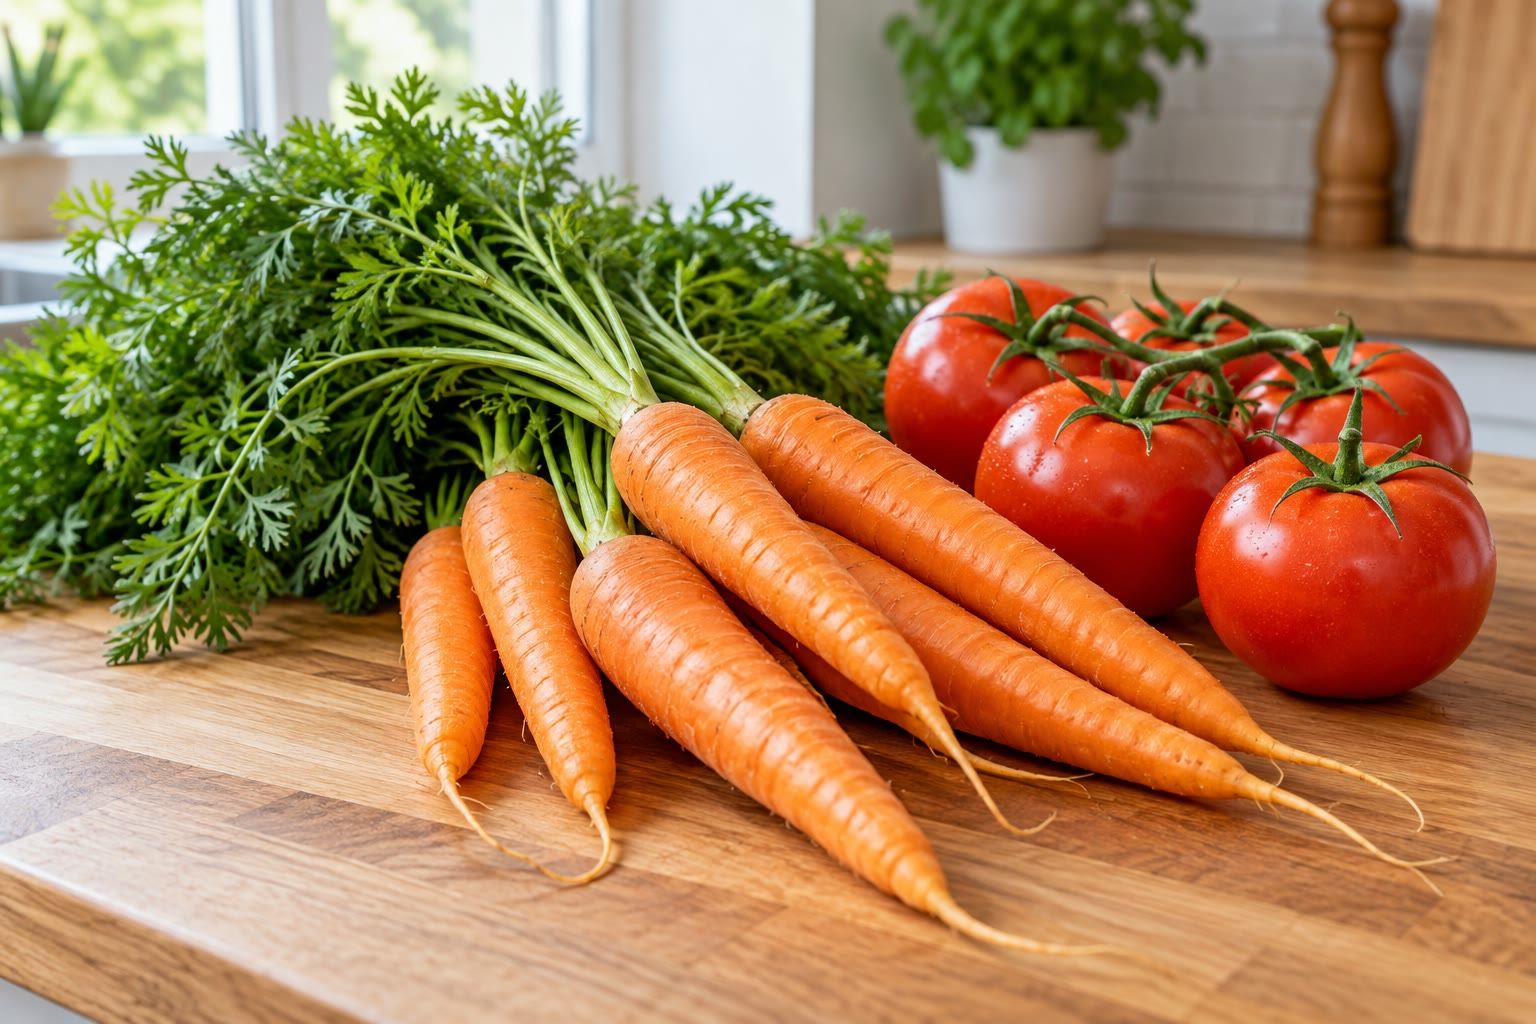
\includegraphics[width=0.55\linewidth]{images/book2/ai/b1-17-carrots-tomatoes.jpg}

{\small गाजर और टमाटर अपने रंग लंबे संयुग्मित अणुओं, कैरोटीनों और
लाइकोपीन, से पाते हैं, जो नीला और हरा प्रकाश अवशोषित करते हैं और नारंगी तथा
लाल को गुज़रने देते हैं।}
\end{omfigure}

\begin{omfigure}
\begin{tikzpicture}[font=\small]
  \foreach \a/\c/\n in {90/red/लाल, 30/orange/नारंगी, -30/yellow/पीला, -90/green!70!black/हरा, -150/blue/नीला, 150/violet/बैंगनी} {
    \fill[\c] (0,0) -- (\a-30:1.4) arc[start angle=\a-30, end angle=\a+30, radius=1.4] -- cycle;
    \node at (\a:1.85) {\n};
  }
  \draw[<->, thick] (-150:0.9) -- (30:0.9);
  \node[align=left, anchor=west] at (2.6,0.3) {नीला अवशोषित करता है $\Rightarrow$ नारंगी दिखता है\\(पूरक रंग चक्र के आर-पार\\एक-दूसरे के सामने होते हैं)};
\end{tikzpicture}

{\small एक रंग-चक्र। दिखने वाला रंग अवशोषित रंग का पूरक होता है:
नीले में अवशोषित करने वाला विलयन नारंगी दिखता है।}
\end{omfigure}

\section{अवरक्त स्पेक्ट्रमिकी का गहन अध्ययन}

\begin{definition}[तरंग संख्या, पारगम्यता, अंगुलिछाप क्षेत्र]\label{def:b1:structure-spectroscopy:wavenumber}
अवरक्त स्पेक्ट्रम \emph{तरंग संख्या}\index{तरंग संख्या}
$\tilde\nu = 1/\lambda$ के विरुद्ध आलेखित किए जाते हैं, \unit{cm^{-1}} में, जो फ़ोटॉन की
ऊर्जा के समानुपाती है। कोटि-अक्ष पर \emph{पारगम्यता}\index{पारगम्यता}
$T = I/I_0$ होती है, प्रतिशत में, ताकि पट्ट नीचे की ओर संकेत करें। लगभग
\qty{1500}{cm^{-1}} से नीचे अनेक अतिव्यापी पट्ट, जो किसी एक आबंध के बजाय पूरे
अणु के अभिलक्षण हैं, \emph{अंगुलिछाप
क्षेत्र}\index{अंगुलिछाप क्षेत्र} बनाते हैं।
\end{definition}

कोई आबंध अवरक्त प्रकाश उस आवृत्ति पर अवशोषित करता है जिस पर वह कंपन करता है। जैसे
स्प्रिंग से जुड़े दो द्रव्यमानों के लिए, आबंध जितना कठोर और परमाणु जितने
हल्के, \omterm{def:b1:structure-spectroscopy:wavenumber}{तरंग संख्या} उतनी ऊँची: हाइड्रोजन से आबंध (O--H, C--H)
\qty{2800}{cm^{-1}} से ऊपर, त्रि-आबंध 2200 के पास, द्वि-आबंध
1700--1600 के पास, भारी परमाणुओं के बीच एकल आबंध 1300 से नीचे। सारणी
इस अध्याय के अणुओं के लिए मापी गई स्थितियाँ देती है, गैस \omterm{def:b1:extent-q-and-k:system}{प्रावस्था} में,
जहाँ अणु पृथक होते हैं।

\begin{omfigure}
\begin{tabular}{llr}
\hline
अणु & आबंध & $\tilde\nu$ (\unit{cm^{-1}}) \\
\hline
एथेनॉल & O--H & 3666 \\
एथेनॉल & C--H & 2978 \\
एथेनॉल & C--O & 1060 \\
प्रोपेनोन & C=O & 1738 \\
एथेनोइक अम्ल & O--H & 3582 \\
एथेनोइक अम्ल & C=O & 1788 \\
एथिल एथेनोएट & C=O & 1764 \\
एथिल एथेनोएट & C--O & 1238 \\
\hline
\end{tabular}

\smallskip
{\small गैस-प्रावस्था अवरक्त स्पेक्ट्रमों में पट्टों के उच्चिष्ठ। द्रवों में, \omterm{def:b1:intermolecular-forces-solvents:hbond}{हाइड्रोजन
आबंध} O--H पट्टों को चौड़ा कर देते हैं और उन्हें निम्नतर \omterm{def:b1:structure-spectroscopy:wavenumber}{तरंग संख्याओं} की ओर ले जाते हैं, और
अम्लों के C=O पट्ट अम्ल के जोड़ी बनाने पर नीचे खिसक जाते हैं।}
% ledger: ir:ethanol-OH, ir:ethanol-CH, ir:ethanol-CO, ir:propanone-CO, ir:ethanoic-OH, ir:ethanoic-CO, ir:ethylethanoate-CO, ir:ethylethanoate-COC
\end{omfigure}

\begin{omfigure}
\begin{tikzpicture}
\begin{axis}[name=i1, width=0.86\linewidth, height=3.2cm, xmin=500, xmax=4000, x dir=reverse, ymin=0, ymax=105, ytick={0,50,100}, ylabel={$T$ (\%)}, tick label style={font=\scriptsize}, label style={font=\small}, xticklabels={}]
\addplot[omDef, thick] table[x=nu, y=T] {figdata/out/bachelor-1-spectra-ir-ethanol.dat};
\node[font=\scriptsize, anchor=west] at (axis cs:2600,25) {एथेनॉल};
\end{axis}
\begin{axis}[name=i2, at={(i1.south)}, anchor=north, yshift=-0.25cm, width=0.86\linewidth, height=3.2cm, xmin=500, xmax=4000, x dir=reverse, ymin=0, ymax=105, ytick={0,50,100}, ylabel={$T$ (\%)}, tick label style={font=\scriptsize}, label style={font=\small}, xticklabels={}]
\addplot[omProp, thick] table[x=nu, y=T] {figdata/out/bachelor-1-spectra-ir-propanone.dat};
\node[font=\scriptsize, anchor=west] at (axis cs:2600,25) {प्रोपेनोन};
\end{axis}
\begin{axis}[at={(i2.south)}, anchor=north, yshift=-0.25cm, width=0.86\linewidth, height=3.2cm, xmin=500, xmax=4000, x dir=reverse, ymin=0, ymax=105, ytick={0,50,100}, ylabel={$T$ (\%)}, tick label style={font=\scriptsize}, label style={font=\small}, xlabel={तरंग संख्या (\unit{cm^{-1}})}]
\addplot[omMeth, thick] table[x=nu, y=T] {figdata/out/bachelor-1-spectra-ir-ethanoic.dat};
\node[font=\scriptsize, anchor=west] at (axis cs:2600,25) {एथेनोइक अम्ल};
\end{axis}
\end{tikzpicture}

{\small एथेनॉल, प्रोपेनोन और एथेनोइक अम्ल के अवरक्त स्पेक्ट्रम,
सारणी की मापी गई पट्ट-स्थितियों से अनुकारित (पट्टों की ऊँचाइयाँ और
चौड़ाइयाँ योजनात्मक)। \qty{1750}{cm^{-1}} के पास का C=O पट्ट और
\qty{3500}{cm^{-1}} से ऊपर का O--H पट्ट तीनों क्रियात्मक समूहों को एक नज़र में
अलग कर देते हैं।}
\end{omfigure}

\section{प्रोटॉन NMR: रासायनिक विस्थापन और समाकलन}

प्रबल चुंबकीय क्षेत्र में प्रोटॉन के दो \omterm{def:b1:quantum-numbers:energy-level}{ऊर्जा स्तर} होते हैं; उचित आवृत्ति की
रेडियो तरंगें उसे एक से दूसरे में पलट देती हैं। वह आवृत्ति
उस चुंबकीय क्षेत्र के समानुपाती है जो प्रोटॉन वास्तव में अनुभव करता है, और जिसे
उसके चारों ओर के इलेक्ट्रॉन थोड़ा घटा देते हैं। इसलिए भिन्न रासायनिक
परिवेशों के प्रोटॉन थोड़ी भिन्न आवृत्तियों पर अनुनाद करते हैं।

\begin{definition}[रासायनिक विस्थापन, परिरक्षण, तुल्य प्रोटॉन]\label{def:b1:structure-spectroscopy:chemical-shift}
किसी प्रोटॉन का \emph{रासायनिक विस्थापन}\index{रासायनिक विस्थापन}
$\delta = (\nu - \nu_{\text{संदर्भ}})/\nu_0 \times 10^6$ है, \unit{ppm} में, जहाँ
$\nu$ उसकी अनुनाद आवृत्ति है, $\nu_{\text{संदर्भ}}$ टेट्रामेथिलसिलेन के प्रोटॉनों की
अनुनाद आवृत्ति और $\nu_0$ स्पेक्ट्रममापी की
प्रचालन आवृत्ति। किसी नाभिक पर उसके इलेक्ट्रॉनों द्वारा क्षेत्र में की गई कमी
उसका \emph{परिरक्षण}\index{परिरक्षण} है: इलेक्ट्रॉन-आकर्षी पड़ोसी
(O, हैलोजन, C=O) प्रोटॉन का विपरिरक्षण करते हैं और उसका $\delta$ बढ़ा देते हैं।
\emph{तुल्य प्रोटॉन}\index{तुल्य प्रोटॉन} वे प्रोटॉन हैं जो अणु की किसी
सममिति से या किसी तीव्र घूर्णन से परस्पर बदल जाते हैं; उनका विस्थापन
समान होता है।
\end{definition}

\begin{proposition}[विस्थापन स्पेक्ट्रममापी पर निर्भर नहीं करता]\label{prop:b1:structure-spectroscopy:shift-field-independent}
किसी प्रोटॉन का \omterm{def:b1:structure-spectroscopy:chemical-shift}{रासायनिक विस्थापन} भिन्न क्षेत्रों वाले स्पेक्ट्रममापियों पर
समान होता है।
\end{proposition}

\begin{proof}
$\nu$ और $\nu_{\text{संदर्भ}}$ दोनों आरोपित क्षेत्र
$B_0$ के समानुपाती हैं (प्रत्येक अपने \omterm{def:b1:structure-spectroscopy:chemical-shift}{परिरक्षण} गुणक से गुणित), और $\nu_0$ भी।
इसलिए अनुपात $(\nu - \nu_{\text{संदर्भ}})/\nu_0$, $B_0$ से
स्वतंत्र है। इसके विपरीत, हर्ट्ज़ में अंतर क्षेत्र के साथ बढ़ते हैं।
\end{proof}

\begin{definition}[समाकलन]\label{def:b1:structure-spectroscopy:integration}
किसी संकेत का \emph{समाकलन}\index{समाकलन} उसका क्षेत्रफल है, जो
स्पेक्ट्रम पर एक सोपान-वक्र की ऊँचाई के रूप में पढ़ा जाता है; क्षेत्रफल
संकेत देने वाले प्रोटॉनों की संख्याओं के समानुपाती होते हैं।
\end{definition}

\section{चक्रण--चक्रण युग्मन}

\begin{definition}[चक्रण--चक्रण युग्मन, युग्मन स्थिरांक, बहुक]\label{def:b1:structure-spectroscopy:coupling}
आबंधों के माध्यम से, किसी प्रोटॉन की चुंबकीय अवस्था पड़ोसी कार्बनों के प्रोटॉनों
द्वारा अनुभव किए गए क्षेत्र को थोड़ा बदल देती है: यह
\emph{चक्रण--चक्रण युग्मन}\index{चक्रण--चक्रण युग्मन} हर संकेत को
रेखाओं के एक \emph{बहुक}\index{बहुक} में विभक्त कर देता है, जो
\emph{युग्मन स्थिरांक}\index{युग्मन स्थिरांक} $J$ से, हर्ट्ज़ में, पृथक होती हैं। एक-दूसरे से
युग्मित दो प्रोटॉन समान $J$ दर्शाते हैं; \omterm{def:b1:structure-spectroscopy:chemical-shift}{तुल्य प्रोटॉन} एक-दूसरे के संकेत को
विभक्त नहीं करते।
\end{definition}

\begin{proposition}[\texorpdfstring{$n + 1$}{n + 1} नियम]\label{prop:b1:structure-spectroscopy:n-plus-one}
समान $J$ से
$n$ तुल्य पड़ोसियों से युग्मित कोई प्रोटॉन (या \omterm{def:b1:structure-spectroscopy:chemical-shift}{तुल्य प्रोटॉनों} का समुच्चय) $n + 1$ रेखाएँ देता है, जो $J$ से पृथक होती हैं और जिनकी
आपेक्षिक तीव्रताएँ द्विपद गुणांक $\binom{n}{k}$ होती हैं, $k = 0$ से
$n$ तक (\emph{$n + 1$ नियम}\index{$n + 1$ नियम})।
\end{proposition}

\begin{proof}
हर पड़ोसी दो चक्रण अवस्थाओं में से किसी एक में होता है, जो प्रेक्षित रेखा को
$+J/2$ या $-J/2$ खिसका देती है। $n$ पड़ोसियों के साथ विस्थापन $(k - n/2)J$ है, जहाँ $k$
पहली अवस्था वाले पड़ोसियों की संख्या है: $n + 1$ मान, $J$ के समान अंतराल पर।
दोनों अवस्थाएँ लगभग समान रूप से आबाद होने के कारण, सभी $2^n$ संयोजन
समान रूप से संभाव्य हैं, और उनमें से $k$ का पहली अवस्था में होना
$\binom{n}{k}$ ढंगों से होता है।
\end{proof}

\begin{omfigure}
\begin{tikzpicture}[font=\small, x=0.85cm, y=0.5cm]
  % quartet: three neighbours, each split +-J/2 (J = 1.5 units)
  \draw[thick] (0,4) -- (0,3.4);
  \foreach \x in {-0.75,0.75} \draw (0,3.4) -- (\x,2.4);
  \foreach \a/\b in {-0.75/-1.5, -0.75/0, 0.75/0, 0.75/1.5} \draw (\a,2.4) -- (\b,1.4);
  \foreach \a/\b in {-1.5/-2.25, -1.5/-0.75, 0/-0.75, 0/0.75, 1.5/0.75, 1.5/2.25} \draw (\a,1.4) -- (\b,0.4);
  \foreach \x/\h in {-2.25/1, -0.75/3, 0.75/3, 2.25/1} {\draw[omDef, very thick] (\x,-2.6) -- (\x,{-2.6+0.7*\h}); \draw[dotted] (\x,0.4) -- (\x,{-2.6+0.7*\h});}
  \draw (-2.8,-2.6) -- (2.8,-2.6);
  \node at (0,-3.4) {चतुष्क 1\,:\,3\,:\,3\,:\,1 (\ce{-CH2-}, \ce{-CH3} के पास)};
  % triplet: two neighbours
  \begin{scope}[xshift=7.5cm]
  \draw[thick] (0,4) -- (0,3.4);
  \foreach \x in {-0.75,0.75} \draw (0,3.4) -- (\x,2.4);
  \foreach \a/\b in {-0.75/-1.5, -0.75/0, 0.75/0, 0.75/1.5} \draw (\a,2.4) -- (\b,1.4);
  \foreach \x/\h in {-1.5/1, 0/2, 1.5/1} {\draw[omProp, very thick] (\x,-2.6) -- (\x,{-2.6+0.7*\h}); \draw[dotted] (\x,1.4) -- (\x,{-2.6+0.7*\h});}
  \draw (-2.1,-2.6) -- (2.1,-2.6);
  \draw[<->] (-1.5,-0.6) -- (0,-0.6) node[midway, above, font=\scriptsize] {$J$};
  \node at (0,-3.4) {त्रिक 1\,:\,2\,:\,1 (\ce{-CH3}, \ce{-CH2-} के पास)};
  \end{scope}
\end{tikzpicture}

{\small विपाटन-वृक्ष। हर पड़ोसी हर रेखा को दो में विभक्त करता है, $J$
की दूरी पर; संपाती रेखाएँ जुड़ जाती हैं, जिससे द्विपद तीव्रताएँ मिलती हैं।}
\end{omfigure}

\begin{omfigure}
\begin{tikzpicture}
\begin{axis}[name=ea,
  width=0.86\linewidth, height=4.2cm, xmin=0.8, xmax=4.5, x dir=reverse, ymin=0, ymax=1.15,
  axis x line=bottom, axis y line=none, xlabel={$\delta$ (ppm)},
  tick label style={font=\scriptsize}, label style={font=\small}]
\addplot[omDef, thin] table[x=ppm, y=I] {figdata/out/bachelor-1-spectra-nmr-ethylethanoate.dat};
\node[font=\scriptsize, anchor=south] at (axis cs:4.12,0.75) {q, 2H};
\node[font=\scriptsize, anchor=west] at (axis cs:2.0,0.95) {s, 3H};
\node[font=\scriptsize, anchor=west] at (axis cs:1.15,0.8) {t, 3H};
\node[font=\small, anchor=north] at (axis cs:3.0,1.1) {\ce{CH3COOCH2CH3}};
\end{axis}
\begin{axis}[at={(ea.south)}, anchor=north, yshift=-1.3cm,
  width=0.86\linewidth, height=4.2cm, xmin=0.8, xmax=4.5, x dir=reverse, ymin=0, ymax=1.15,
  axis x line=bottom, axis y line=none, xlabel={$\delta$ (ppm)},
  tick label style={font=\scriptsize}, label style={font=\small}]
\addplot[omProp, thin] table[x=ppm, y=I] {figdata/out/bachelor-1-spectra-nmr-ethanol.dat};
\node[font=\scriptsize, anchor=south] at (axis cs:3.69,0.75) {q, 2H};
\node[font=\scriptsize, anchor=west] at (axis cs:2.55,0.6) {s, 1H};
\node[font=\scriptsize, anchor=west] at (axis cs:1.1,0.8) {t, 3H};
\node[font=\small, anchor=north] at (axis cs:2.9,1.1) {\ce{CH3CH2OH}};
\end{axis}
\end{tikzpicture}

{\small \ce{CDCl3} में एथिल एथेनोएट (ऊपर) और एथेनॉल (नीचे) के प्रोटॉन NMR स्पेक्ट्रम (q: चतुष्क, s: एकक, t: त्रिक),
मापे गए विस्थापनों और \omterm{def:b1:structure-spectroscopy:coupling}{युग्मन स्थिरांकों} से \qty{90}{MHz} पर अनुकारित
($J = \qty{7.2}{Hz}$ और \qty{7.0}{Hz})।
\ce{OCH2} चतुष्क ऑक्सीजन द्वारा विपरिरक्षित है; एथेनॉल में OH प्रोटॉन,
जो अणुओं के बीच तेज़ी से विनिमित होता है, युग्मित नहीं होता और उसका विस्थापन
सांद्रता पर निर्भर करता है।}
% ledger: nmr:ethylethanoate-OCH2, nmr:ethylethanoate-COCH3, nmr:ethylethanoate-CH3, nmr:ethylethanoate-J, nmr:ethanol-CH2, nmr:ethanol-CH3, nmr:ethanol-OH, nmr:ethanol-J
\end{omfigure}

\begin{omfigure}
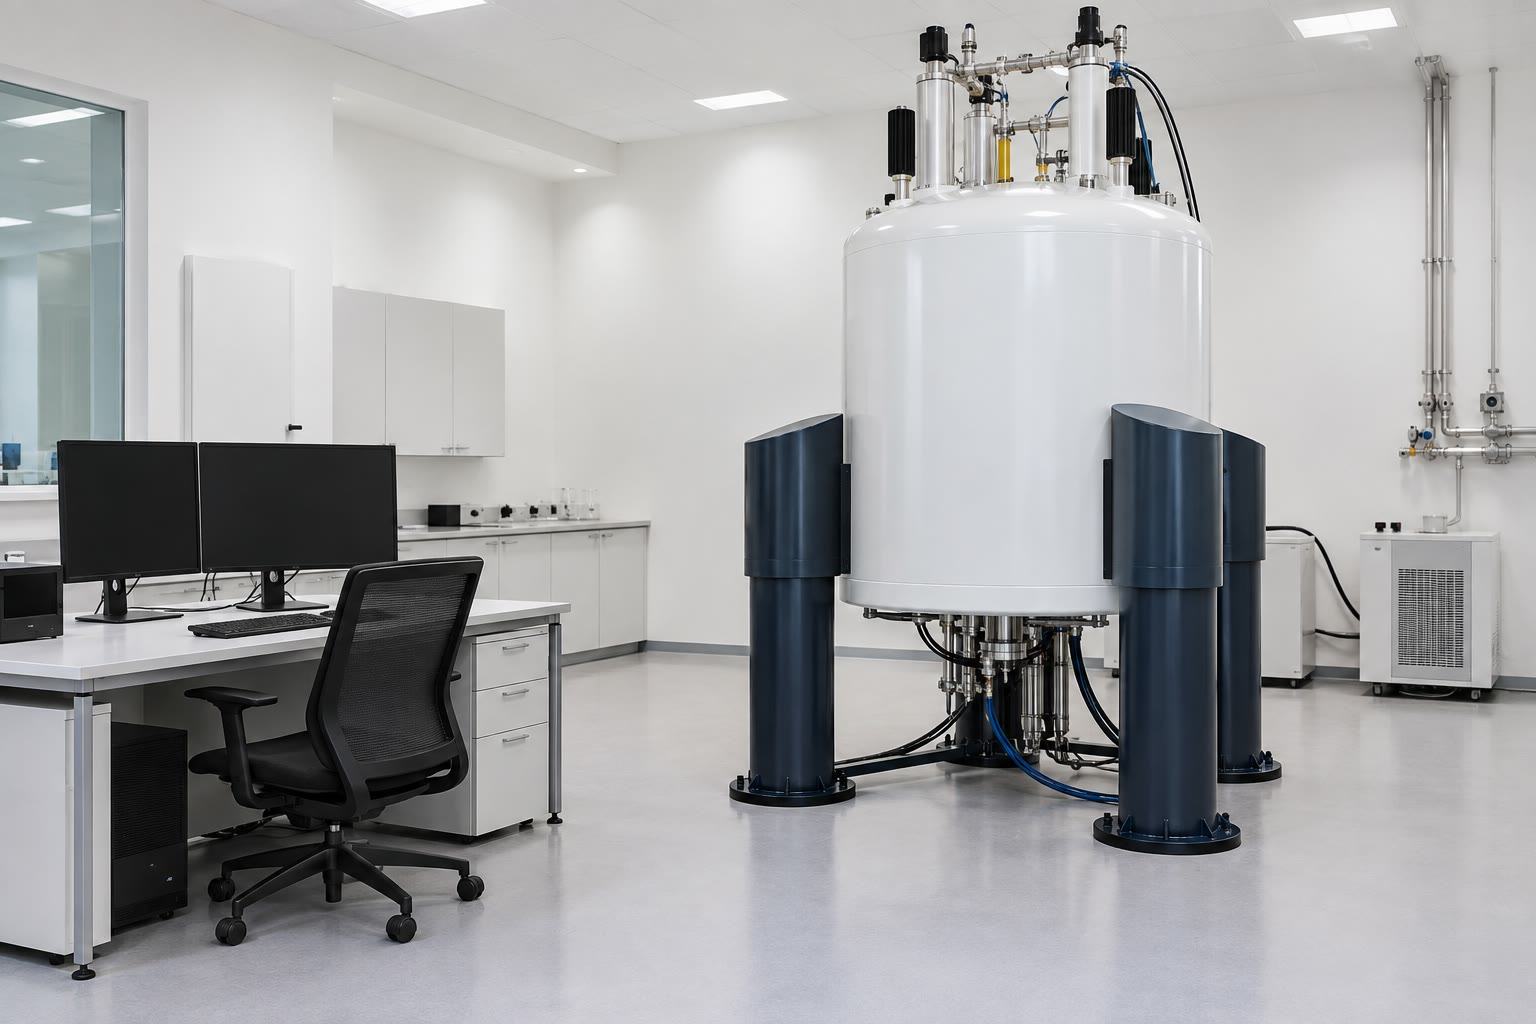
\includegraphics[width=0.5\linewidth]{images/book2/ai/b1-17-nmr.jpg}

{\small एक NMR स्पेक्ट्रममापी: ऊँचे बेलन में द्रव हीलियम से ठंडा किया गया
अतिचालक चुंबक है; नमूना-नली को उसके केंद्र में
नीचे उतारा जाता है।}
\end{omfigure}

\section{संरचना ज्ञात करना}

\begin{definition}[असंतृप्ति की मात्रा]\label{def:b1:structure-spectroscopy:unsaturation}
किसी सूत्र की \emph{असंतृप्ति की मात्रा}\index{असंतृप्ति की मात्रा}
अणु में वलयों की संख्या और $\pi$ आबंधों की संख्या का
योग है।
\end{definition}

\begin{proposition}[सूत्र से असंतृप्ति की मात्रा]\label{prop:b1:structure-spectroscopy:unsaturation-formula}
अणु $\mathrm{C}_c\mathrm{H}_h\mathrm{N}_n\mathrm{O}_o\mathrm{X}_x$
(X एक हैलोजन) के लिए \omterm{def:b1:structure-spectroscopy:unsaturation}{असंतृप्ति की मात्रा} है
\[
  D = \frac{2c + 2 + n - h - x}{2} .
\]
\end{proposition}

\begin{proof}
केवल एकल आबंधों वाली $c$ कार्बनों की खुली शृंखला पर $2c + 2$
हाइड्रोजन होते हैं। हर वलय या $\pi$ आबंध उनमें से दो हटा देता है। शृंखला में
डाला गया द्विसंयोजी ऑक्सीजन कुछ नहीं बदलता; त्रिसंयोजी नाइट्रोजन एक और
हाइड्रोजन लाता है; हैलोजन एक हाइड्रोजन का स्थान लेता है। कम पड़ने वाले
हाइड्रोजनों को गिनकर दो से भाग देने पर $D$ मिलता है।
\end{proof}

\begin{method}[संरचना ज्ञात करना]\label{met:b1:structure-spectroscopy:solve-structure}
\begin{enumerate}
  \item सूत्र से $D$ परिकलित कीजिए।
  \item अवरक्त स्पेक्ट्रम से क्रियात्मक समूह (C=O, O--H, N--H,
        C--O) और अन्य समूहों की अनुपस्थिति ज्ञात कीजिए।
  \item NMR स्पेक्ट्रम से: संकेतों की संख्या (\omterm{def:b1:structure-spectroscopy:chemical-shift}{तुल्य प्रोटॉनों} के
        समुच्चय), \omterm{def:b1:structure-spectroscopy:integration}{समाकलन} (प्रति समुच्चय प्रोटॉन), विस्थापन (पड़ोसी
        समूह), बहुकता (पड़ोसियों की संख्या, $n + 1$
        नियम से), \omterm{def:b1:structure-spectroscopy:coupling}{युग्मन स्थिरांक} (कौन-से संकेत पड़ोसी हैं)।
  \item खंड बनाइए, उन्हें जोड़िए, और हर शिखर की प्रस्तावित संरचना से
        जाँच कीजिए; असहमत समावयवियों को त्याग दीजिए।
\end{enumerate}
\end{method}

\section{अभ्यास}

\begin{exercise}[$\star$]\label{exo:b1:structure-spectroscopy:1}
\qty{1.00}{cm} के सेल में \qty{2.0e-5}{mol/L} पर एक रंजक के विलयन की
\omterm{def:b1:structure-spectroscopy:conjugation}{अवशोषण उच्चिष्ठ} पर \omterm{def:b1:structure-spectroscopy:absorbance}{अवशोषकता} 0.64 है। $\varepsilon$ परिकलित कीजिए, और
तीन गुना अधिक सांद्र विलयन की \omterm{def:b1:structure-spectroscopy:absorbance}{अवशोषकता} भी।
\end{exercise}

\begin{exercise}[$\star$]\label{exo:b1:structure-spectroscopy:2}
\ce{C6H6}, \ce{C4H8O2}, \ce{C3H7NO},
\ce{C2H3Cl} और \ce{C10H14O} (कार्वोन) की \omterm{def:b1:structure-spectroscopy:unsaturation}{असंतृप्ति की मात्रा} परिकलित कीजिए। हर एक के लिए एक संरचना प्रस्तावित कीजिए।
\end{exercise}

\begin{exercise}[$\star$]\label{exo:b1:structure-spectroscopy:3}
प्रोपेनोन, एथेनोइक
अम्ल, 2-मेथिलप्रोपेन और 1,2-डाइक्लोरोएथेन कितने प्रोटॉन संकेत देते हैं, और किन \omterm{def:b1:structure-spectroscopy:integration}{समाकलनों} के साथ?
\end{exercise}

\begin{exercise}[$\star$]\label{exo:b1:structure-spectroscopy:4}
एक संकेत \qty{400}{MHz} स्पेक्ट्रममापी पर टेट्रामेथिलसिलेन से \qty{1460}{Hz} दूर
स्थित है। उसका विस्थापन क्या है? \qty{90}{MHz} पर वह हर्ट्ज़ में कितनी दूर
होता? ऊँचे क्षेत्र \omterm{def:b1:structure-spectroscopy:coupling}{बहुकों} को बेहतर पृथक क्यों करते हैं?
\end{exercise}

\begin{exercise}[$\star\star$]\label{exo:b1:structure-spectroscopy:5}
1-ब्रोमोप्रोपेन, \ce{CH3CH2CH2Br}, के हर संकेत की बहुकता का पूर्वानुमान कीजिए,
\omterm{def:b1:structure-spectroscopy:coupling}{युग्मन स्थिरांकों} को बराबर मानकर, और केंद्रीय संकेत की रेखाओं की आपेक्षिक
तीव्रताएँ भी बताइए।
\end{exercise}

\begin{exercise}[$\star\star$]\label{exo:b1:structure-spectroscopy:6}
1700 और \qty{3700}{cm^{-1}} के बीच एथेनॉल, प्रोपेनोन और एथेनोइक अम्ल के अवरक्त
स्पेक्ट्रम कैसे भिन्न हैं? कौन-सा एक यौगिक C=O और O--H
दोनों पट्ट देता है?
\end{exercise}

\begin{exercise}[$\star\star$]\label{exo:b1:structure-spectroscopy:7}
\ce{C4H8O2} के दो समावयवी: एथिल एथेनोएट और मेथिल प्रोपेनोएट। उनके
NMR स्पेक्ट्रमों (लगभग विस्थापन, बहुकता, \omterm{def:b1:structure-spectroscopy:integration}{समाकलन}) का पूर्वानुमान कीजिए
और बताइए कि उन्हें कैसे अलग पहचाना जाए।
\end{exercise}

\begin{exercise}[$\star\star$]\label{exo:b1:structure-spectroscopy:8}
एथिल एथेनोएट के अनुकारित स्पेक्ट्रम का उपयोग करके, चतुष्क की दो रेखाओं के बीच का
अंतराल ppm में पढ़िए और उसे हर्ट्ज़ में बदलिए (स्पेक्ट्रम
\qty{90}{MHz} पर अनुकारित है)। त्रिक से तुलना कीजिए।
\end{exercise}

\begin{exercise}[$\star\star$]\label{exo:b1:structure-spectroscopy:9}
एक यौगिक \ce{C3H6O} \qty{1738}{cm^{-1}} पर एक प्रबल अवरक्त पट्ट और
एक ही NMR संकेत दर्शाता है। उसे पहचानिए। कौन-सा समावयवी
\qty{2720}{cm^{-1}} के पास एक पट्ट और \qty{9.8}{ppm} के पास एक संकेत दर्शाएगा?
\end{exercise}

\begin{exercise}[$\star\star\star$]\label{exo:b1:structure-spectroscopy:10}
$n + 1$ नियम को इस रूप में सिद्ध कीजिए: पड़ोसियों के दो भिन्न
समुच्चयों से युग्मित प्रोटॉन, $n_1$ से $J_1$ के साथ और $n_2$ से $J_2$ के साथ, $(n_1 +
1)(n_2 + 1)$ रेखाएँ देता है। जब $J_1 = J_2$ हो, तब कितनी भिन्न रेखाएँ बचती हैं?
इसे 1-ब्रोमोप्रोपेन के केंद्रीय \ce{CH2} पर लागू कीजिए।
\end{exercise}

\begin{exercise}[$\star\star\star$]\label{exo:b1:structure-spectroscopy:11}
एक यौगिक \ce{C4H10O} 1700--1800 पर कोई अवरक्त पट्ट नहीं देता, पर द्रव में
\qty{3350}{cm^{-1}} के पास एक चौड़ा पट्ट देता है, और ऐसा NMR स्पेक्ट्रम जिसमें एक द्विक
(6H), एक \omterm{def:b1:structure-spectroscopy:coupling}{बहुक} (1H), एक द्विक (2H) और एक चौड़ा एकक (1H) है।
संरचना ज्ञात कीजिए।
\end{exercise}

\begin{exercise}[$\star\star\star$]\label{exo:b1:structure-spectroscopy:12}
दिखाइए कि दो स्पीशीज़ के मिश्रण की \omterm{def:b1:structure-spectroscopy:absorbance}{अवशोषकता} $A = \ell(\varepsilon_1c_1
+ \varepsilon_2c_2)$ का पालन करती है, और समझाइए कि दो तरंगदैर्घ्यों पर मापन
दोनों सांद्रताएँ कैसे देते हैं।
\end{exercise}

\section{समस्या: अनन्नास वाला अणु}

\begin{problem}[{सप्ताहांत समस्या --- दहन विश्लेषण और वाष्प
घनत्व, अवरक्त स्पेक्ट्रम, प्रोटॉन NMR स्पेक्ट्रम, और
अनन्नास की गंध वाले एस्टर की संरचना और मोलर द्रव्यमान}]
\label{pb:b1:structure-spectroscopy:1}
अज्ञात पदार्थ एक द्रव है जिसमें केवल C, H और O हैं।
\qty{0.2500}{g} के दहन से \qty{0.5690}{g} कार्बन डाइऑक्साइड और
\qty{0.2328}{g} जल मिलता है। उसके वाष्प का घनत्व \qty{100}{\celsius} और
\qty{1.000}{bar} पर \qty{3.74}{g/L} है। गैस-प्रावस्था अवरक्त पट्ट: 2982,
1754, \qty{1182}{cm^{-1}} (प्रबल), \qty{3100}{cm^{-1}} से ऊपर
कोई नहीं। प्रोटॉन NMR (\ce{CDCl3}): 4.13 (चतुष्क, 2H, $J = \qty{7.2}{Hz}$),
2.28 (त्रिक, 2H), 1.66 (षष्टक, 2H), 1.25 (त्रिक, 3H, $J = \qty{7.2}{Hz}$), 0.95
(त्रिक, 3H) ppm। $M$: C 12.0, H 1.0, O \qty{16.0}{g/mol}; $R =
\qty{8.314}{J/(K.mol)}$।
% ledger: ir:ethylbutanoate-CH, ir:ethylbutanoate-CO, ir:ethylbutanoate-COC, nmr:ethylbutanoate-OCH2, nmr:ethylbutanoate-CH2CO, nmr:ethylbutanoate-CH2, nmr:ethylbutanoate-OCH2CH3, nmr:ethylbutanoate-CH3, nmr:ethylbutanoate-J

\begin{center}
\begin{tikzpicture}
\begin{axis}[width=0.86\linewidth, height=4.0cm, xmin=0.6, xmax=4.5, x dir=reverse, ymin=0, ymax=1.15,
  axis x line=bottom, axis y line=none, xlabel={$\delta$ (ppm)},
  tick label style={font=\scriptsize}, label style={font=\small}]
\addplot[omDef, thin] table[x=ppm, y=I] {figdata/out/bachelor-1-spectra-nmr-ethylbutanoate.dat};
\end{axis}
\end{tikzpicture}
\end{center}

\medskip
\noindent\textbf{भाग I --- सूत्र।}
\begin{enumerate}
  \item नमूने में कार्बन का द्रव्यमान परिकलित कीजिए।
  \item हाइड्रोजन का द्रव्यमान परिकलित कीजिए।
  \item ऑक्सीजन का द्रव्यमान निकालिए।
  \item C, H और O के द्रव्यमान प्रतिशत परिकलित कीजिए।
  \item मूलानुपाती सूत्र ज्ञात कीजिए।
  \item वाष्प घनत्व से मोलर द्रव्यमान परिकलित कीजिए (आदर्श गैस)।
  \item आण्विक सूत्र और उसकी \omterm{def:b1:structure-spectroscopy:unsaturation}{असंतृप्ति की मात्रा} बताइए।
\end{enumerate}

\medskip
\noindent\textbf{भाग II --- अवरक्त स्पेक्ट्रम।}
\begin{enumerate}[resume]
  \item \qty{1754}{cm^{-1}} के पट्ट का निर्धारण कीजिए।
  \item \qty{3100}{cm^{-1}} से ऊपर पट्टों की अनुपस्थिति किसे वर्जित करती है?
  \item \qty{1182}{cm^{-1}} के प्रबल पट्ट का निर्धारण कीजिए।
  \item \qty{2982}{cm^{-1}} के पट्ट का निर्धारण कीजिए।
  \item \omterm{def:b1:structure-spectroscopy:unsaturation}{असंतृप्ति की मात्रा} को देखते हुए, यौगिकों का कौन-सा कुल
        बचता है? कार्बोक्सिलिक अम्ल, ईथर-युक्त कीटोन, या
        चक्रीय डाइऑल क्यों नहीं?
\end{enumerate}

\medskip
\noindent\textbf{भाग III --- NMR स्पेक्ट्रम।}
\begin{enumerate}[resume]
  \item \omterm{def:b1:structure-spectroscopy:chemical-shift}{तुल्य प्रोटॉनों} के कितने समुच्चय हैं? कुल \omterm{def:b1:structure-spectroscopy:integration}{समाकलन} की जाँच कीजिए।
  \item 4.13 ppm पर चतुष्क की व्याख्या कीजिए: पड़ोसी और परिवेश।
  \item 1.25 ppm पर त्रिक की व्याख्या कीजिए। दोनों का
        $J$ समान क्यों है?
  \item 2.28 ppm पर त्रिक की व्याख्या कीजिए।
  \item 1.66 ppm पर षष्टक की व्याख्या कीजिए।
  \item 0.95 ppm पर त्रिक की व्याख्या कीजिए।
  \item वे दो खंड बनाइए जिनका वर्णन ये संकेत करते हैं।
  \item 4.13 और 2.28 ppm के संकेत सबसे अधिक विपरिरक्षित क्यों हैं?
\end{enumerate}

\medskip
\noindent\textbf{भाग IV --- संरचना।}
\begin{enumerate}[resume]
  \item खंडों को एस्टर समूह के माध्यम से जोड़िए: दो संभावनाएँ।
        कौन-सी विस्थापनों से संगत है?
  \item समझाइए कि प्रोपिल प्रोपेनोएट क्यों उपयुक्त नहीं है।
  \item समझाइए कि ब्यूटिल एथेनोएट क्यों उपयुक्त नहीं है।
  \item यौगिक का नाम बताइए और उसकी संरचना खींचिए।
  \item हर अवरक्त पट्ट और हर NMR संकेत की संरचना से जाँच कीजिए।
  \item अनन्नास वाले अणु का मोलर द्रव्यमान बताइए।
\end{enumerate}
\end{problem}
